% ===============================================================
% Document Class ================================================
\documentclass{article}

% ===============================================================
% Graphic Packages ==============================================
\usepackage{graphicx}       % Permite a inclusão de imagens no documento.
\usepackage{tikz}           % Ferramenta poderosa para criar gráficos programaticamente dentro do LaTeX.
\usetikzlibrary{calc}       % Extensão da biblioteca TikZ que permite cálculos mais complexos de coordenadas.

% ===============================================================
% Mathematical Tools ============================================
\usepackage{amsmath}        % Melhora a aparência e a flexibilidade de comandos matemáticos.
\usepackage{siunitx}        % Facilita o uso de unidades do Sistema Internacional e ajuda a formatar números complexos.

% ===============================================================
% Font and Text Appearance ======================================
\usepackage{mathptmx}       % Altera a fonte padrão do documento para Times New Roman.

% ===============================================================
% Table of Contents Customization ===============================
\usepackage{tocloft}  % Oferece controle total sobre a aparência das listas de conteúdos, figuras, tabelas, etc.

% ===============================================================
% Figure Positioning ============================================
\usepackage{float}     % Melhora a interface para definir o posicionamento de objetos flutuantes como figuras e tabelas.

% ===============================================================
% Paragraph Spacing and Indentation =============================
\usepackage{setspace}  % Permite o ajuste fino do espaçamento entre linhas.
\usepackage{indentfirst} % Adiciona indentação ao primeiro parágrafo de cada seção.

% ===============================================================
% Page Layout ===================================================
\usepackage[a4paper, top=3cm, bottom=2cm, left=3cm, right=2cm]{geometry}  % Define as margens de todo o documento.
\setlength{\parindent}{4em}  % Define o tamanho da indentação para todos os parágrafos.

% ===============================================================
% Section Heading Customization =================================
\makeatletter
\renewcommand\paragraph{\@startsection{paragraph}{4}{\z@}%
    {2ex plus 1ex minus .2ex}%
    {1em}%
    {\normalfont\normalsize\bfseries}}
\makeatother


% ===============================================================
% Begin Document ================================================
\begin{document}

% ===============================================================
% Capa ==========================================================
\begin{titlepage}
    \centering
    % Desenhar a margem
    \begin{tikzpicture}[remember picture, overlay]
        \draw[line width = 4pt] ($(current page.north west) + (20mm, -20mm)$) rectangle ($(current page.south east) + (-10mm,10mm)$);
        \draw[line width = 1pt] ($(current page.north west) + (21.5mm,-21.5mm)$) rectangle ($(current page.south east) + (-11.5mm,11.5mm)$);
    \end{tikzpicture}

    % Linha de logos
    
\includegraphics[height=0.151\textwidth]{header/contra-capa/assets/uerj.png}\hfill
    
\includegraphics[height=0.15\textwidth]{header/contra-capa/assets/iprj.jpeg}\hfill

    \vspace{2cm} % Espaço vertical após os logos

    % Informações do curso
    {\Large\bfseries Instituto Politécnico do Estado do Rio de Janeiro \par}
    \vspace{0.5cm}
    {\large Curso de Engenharia da Computação \par}

    \vspace{3cm} % Espaço vertical antes do título da atividade

    % Nome do estudante
    {\large\bfseries Guilherme Cagide Fialho \par}

    \vspace{3cm}

    % Título da atividade
    {\large\bfseries Projeto de Modelagem e Controle de Sistemas em Scilab \par}

    \vfill % Empurra o restante para o fundo da página

    % Local e ano
    {\large\bfseries Nova Friburgo \par}
    \vspace{0.3cm}
    {\large\bfseries 2024 \par}
\end{titlepage}
\newpage % Começa uma nova página após a capa


% ===============================================================
% Contra Capa ===================================================
\begin{titlepage}
    \centering
    % Desenhar a margem
    \begin{tikzpicture}[remember picture, overlay]
        \draw[line width = 4pt] ($(current page.north west) + (20mm, -20mm)$) rectangle ($(current page.south east) + (-10mm,10mm)$);
        \draw[line width = 1pt] ($(current page.north west) + (21.5mm,-21.5mm)$) rectangle ($(current page.south east) + (-11.5mm,11.5mm)$);
    \end{tikzpicture}

    % Linha de logos
    
\includegraphics[height=0.151\textwidth]{header/contra-capa/assets/uerj.png}\hfill
    
\includegraphics[height=0.15\textwidth]{header/contra-capa/assets/iprj.jpeg}\hfill

    \vspace{2cm} % Espaço vertical após os logos

    % Informações do curso
    {\Large\bfseries Instituto Politécnico do Estado do Rio de Janeiro \par}
    \vspace{0.5cm}
    {\large Graduação em Engenharia da Computação \par}

    \vspace{3cm} % Espaço vertical antes do título da atividade

    % Nome do estudante
    {\large Guilherme Cagide Fialho \par}

    \vspace{1.5cm}

    % Título da atividade
    {\large\bfseries Projeto de Modelagem e Controle de Sistemas em Scilab \par}

    \vspace{1cm} % Espaço vertical antes do título da atividade

    % Informações do projeto
    \begin{flushright}
        \begin{minipage}{0.5\textwidth}
            \large
            \raggedleft % Garante que o texto dentro da minipage seja alinhado à direita
            Projeto de Conclusão da Disciplina Modelagem e Controle de Sistemas
        \end{minipage}
    \end{flushright}

    \vspace{1.5cm}

    % Informações do orientador
    \begin{flushleft}
        \begin{minipage}{0.5\textwidth}
            \large
            \raggedright
            Orientador: Prof. Joel Sánchez Domínguez
        \end{minipage}
    \end{flushleft}


    \vfill % Empurra o restante para o fundo da página

    % Local e ano
    {\large Nova Friburgo \par}
    \vspace{0.3cm}
    {\large 2024 \par}
\end{titlepage}
\newpage % Começa uma nova página após a capa


% ===============================================================
% Resumo ========================================================
% \begin{titlepage}
    \thispagestyle{empty} % Remove números de página
    \setstretch{1.5} % Espaçamento entre linhas, certifique-se de que o pacote setspace está incluído em document.tex

    \begin{center}
        \textbf{\Large RESUMO}
    \end{center}


    \vspace{1cm} % Espaço vertical

    \noindent CAGIDE FIALHO, G. Relatório do projeto de Modelagem
    e controle de sistemas. 2024. 54 f. Trabalho de Conclusão de Disciplina Modelagem e Controle de Sistemas (Graduação em
    Engenharia da computação) – Graduação em Engenharia da Computação, Universidade
    do Estado do Rio de Janeiro, Nova Friburgo, 2024.

    \vspace{0.4cm} % Espaço vertical

    Este trabalho explora a modelagem e o controle de um sistema dinâmico do tipo massa-mola-amortecedor, utilizando a plataforma Scilab para desenvolvimento e simulação. O foco do estudo está na implementação de modelos matemáticos para descrever a dinâmica do sistema e na análise de sua resposta sob diversas condições iniciais, sem a aplicação de forças externas. Utilizando a ferramenta Xcos, um componente gráfico do Scilab, realizamos simulações que permitiram uma análise visual e quantitativa das respostas transientes do sistema. O estudo destaca a influência dos parâmetros físicos, como a massa, o coeficiente de amortecimento, e a constante da mola, nas características de resposta do sistema. Além disso, técnicas de controle foram empregadas para ajustar a resposta do sistema, demonstrando como o amortecimento pode contribuir para a estabilização após perturbações e enfatizando a relevância de uma parametrização cuidadosa para alcançar um comportamento eficaz do sistema. Este projeto contribui para a compreensão das teorias de controle aplicáveis em sistemas mecânicos e outros contextos de sistemas dinâmicos na engenharia.
    \vspace{0.4cm} % Espaço vertical

    \textbf{Palavras-chave}: Modelagem e Controle, Sistema Massa-Mola-Amortecedor, Simulação, Scilab, Xcos.
\end{titlepage}


% ===============================================================
% Abstract ======================================================
% \begin{titlepage}
    \thispagestyle{empty} % Remove números de página
    \setstretch{1.5} % Espaçamento entre linhas, certifique-se de que o pacote setspace está incluído em document.tex

    \begin{center}
        \textbf{\Large ABSTRACT}
    \end{center}

    \vspace{1cm} % Espaço vertical

    % \noindent % Garante que o primeiro parágrafo não seja indentado
    % Santos, Leonardo Pereira. \textit{Simulação em Scilab em um sistema massa-mola-amortecedor}, 2023. Projeto de conclusão da disciplina Modelagem e Controle de Sistemas - Instituto Politécnico, Universidade do Estado do Rio de Janeiro, Nova Friburgo, 2023.

    % \vspace{1cm} % Espaço vertical

    % \noindent
    % Neste trabalho, veremos de que modo a ferramenta e linguagem Scilab consegue auxiliar na modelagem de um sistema físico, desde a parte da criação do modelo matemático até a interpretação do comportamento do mesmo por meio de gráficos.

    % \vspace{0.5cm} % Espaço vertical

    % \noindent
    % Palavras-chave: Sistema massa-mola-amortecedor, função de transferência, scilab.
\end{titlepage}


% ===============================================================
% Atividades ====================================================
\section{Atividade 1}
\subsection{Descrição do Modelo}
O sistema modelado é um oscilador massa-mola-amortecedor, onde a massa está sujeita à força restauradora de uma mola e ao amortecimento proporcional à velocidade. A equação diferencial que descreve o movimento do sistema é dada por:
\[
    m \ddot{x} + C \dot{x} + Kx = 0
\]
onde \( x \) representa o deslocamento da massa \( m \) da sua posição de equilíbrio, \( \dot{x} \) é a velocidade, \( \ddot{x} \) é a aceleração, \( C \) é o coeficiente de amortecimento, e \( K \) é a constante da mola. A força de entrada é considerada nula, indicando que não há forças externas atuando sobre o sistema após o instante inicial.

\subsection{Parâmetros do Sistema}
Os parâmetros utilizados no modelo do sistema são especificados como segue:
\begin{itemize}
    \item Massa (\( m \)): 10 kg
    \item Coeficiente de amortecimento (\( C \)): 7 Ns/m
    \item Constante da mola (\( K \)): 5 N/m
\end{itemize}

\subsection{Condições Iniciais para a Simulação}
As condições iniciais para a simulação são detalhadas na tabela a seguir, baseadas nos parâmetros especificados acima:
\begin{center}
    \begin{tabular}{|c|c|c|}
        \hline
        \textbf{Caso} & \textbf{Velocidade Inicial \( V_0 \)} & \textbf{Posição Inicial \( X_0 \)} \\
        \hline
        1             & \( 5 \, \text{m/s} \)                 & \( 0 \, \text{m} \)                \\
        2             & \( 0 \, \text{m/s} \)                 & \( 2.5 \, \text{m} \)              \\
        3             & \( 3.33 \, \text{m/s} \)              & \( 2 \, \text{m} \)                \\
        \hline
    \end{tabular}
\end{center}

Esta tabela reflete os valores numéricos para cada caso, facilitando a compreensão e a aplicação direta dos parâmetros na simulação.

\subsection{Código Scilab para simular a resposta do sistema massa-mola-amortecedor}
Código Scilab utilizado para as análises que serão feitas subsequentes
\begin{lstlisting}[language=Scilab, caption=Código Scilab para simular a resposta do sistema massa-mola-amortecedor]
    // Definicao das principais variaveis do sistema fisico
    m = 10;  // massa
    c = 7;   // coeficiente de amortecimento
    k = 5;   // constante da mola

    // Funcao que define o sistema de equacoes diferenciais (EDO) para o modelo massa-mola-amortecedor
    function dxdt = sistema(t, x)
    // x(1) representa o deslocamento, x(2) representa a velocidade
    // Esta funcao retorna a derivada da velocidade e do deslocamento, respectivamente
    dxdt = [x(2); -c/m * x(2) - k/m * x(1)];
    endfunction

    // Configuracao do intervalo de tempo para a simulacao
    t0 = 0; // Tempo inicial (s)
    tf = 20; // Tempo final (s)
    t = linspace(t0, tf, 1000); // Cria um vetor de tempo linearmente espacado para a simulacao

    // Definicao das condicoes iniciais para cada caso de simulacao
    condicoes_iniciais = [
    m/5, m/3; // Caso 3: posicao inicial (m) e velocidade inicial (m/s)
    m/4, 0;   // Caso 2: posicao inicial (m) e velocidade inicial (m/s)
    0, m/2;   // Caso 1: posicao inicial (m) e velocidade inicial (m/s)
    ];

    // Cores designadas para cada caso de simulacao para facilitar a visualizacao
    cores = ['#007bff', '#dc3545', '#8B4513']; // Azul, vermelho, marrom

    // Loop para executar e plotar cada caso de simulacao separadamente
    for i = 1:3
        x0 = condicoes_iniciais(i, :)'; // Transpoe as condicoes iniciais para a formatacao correta
        sol = ode(x0, t0, t, sistema); // Resolve a EDO usando o metodo de ODE

        scf(i); // Cria uma nova figura para cada iteracao
        plot(t, sol(1, :),  'color', cores(i),  'LineWidth', 2); // Plot do deslocamento x(t)
        xlabel('Tempo (s)'); // Etiqueta do eixo X
        ylabel('Deslocamento x(t)'); // Etiqueta do eixo Y
        title(['Resposta do Sistema para o Caso ', string(i)]); // Titulo do grafico
        legend('x(t)', "location", "best"); // Legenda
        xgrid(); // Ativa a grade no grafico
    end

    // Preparacao do grafico combinado
    scf(); // Cria uma nova figura
    clf(); // Limpa a figura atual
    xlabel('Tempo (s)');
    ylabel('Deslocamento x(t)');
    title('Resposta do Sistema para Todos os Casos');
    xgrid(); // Ativando a grade

    // Execucao da simulacao para cada caso e plotagem no mesmo grafico
    for i = 1:3
    x0 = condicoes_iniciais(i, :)'; // Condicoes iniciais para o caso i (transposto para coluna)
    sol = ode(x0, t0, t, sistema); // Resolvendo a equacao diferencial

    // Plotando os resultados com cores definidas
    plot(t, sol(1, :), 'color', cores(i), 'LineWidth', 2);
    end

    // Criar a legenda detalhando cada caso
    legend(['Caso 1: x0 = 0, v0 = m/2', 'Caso 2: x0 = m/4, v0 = 0', 'Caso 3: x0 = m/5, v0 = m/3'], "location", "best");
\end{lstlisting}

\subsection{Análise dos Resultados}
Cada um dos casos de simulação foi configurado com condições iniciais distintas para explorar como o sistema responde a diferentes estados iniciais de deslocamento e velocidade.

\subsubsection{Caso 1: Velocidade Inicial Elevada}
\begin{figure}[H]
    \centering
    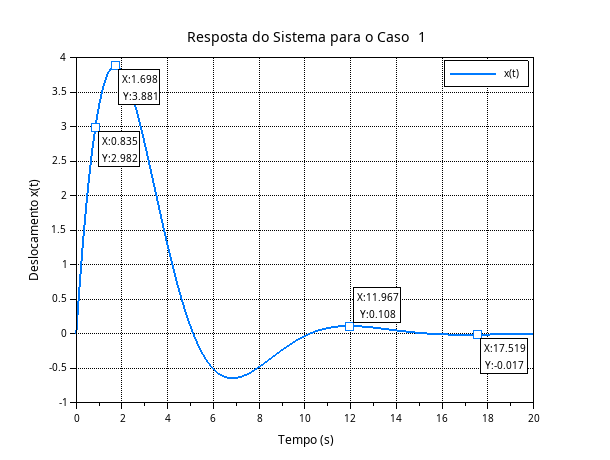
\includegraphics[width=0.6\textwidth]{atividades/1-atividade/assets/caso1.png}
    \caption{Resposta do sistema para o Caso 1}
\end{figure}
No Caso 1, o sistema é inicialmente impulsionado com uma alta velocidade (\(5 \, \text{m/s}\)), partindo do repouso (\(X_0 = 0\)). Esta condição inicial leva a uma resposta inicialmente enérgica, onde a massa oscila com uma amplitude elevada, seguida de um rápido decaimento energético devido ao amortecimento significativo (\(C = 7 \, \text{Ns/m}\)). O amortecimento não só reduz a amplitude das oscilações rapidamente, mas também garante que o sistema não persista em um estado de oscilação prolongada, estabilizando-se em um tempo curto.

\subsubsection{Caso 2: Deslocamento Inicial Sem Velocidade}
\begin{figure}[H]
    \centering
    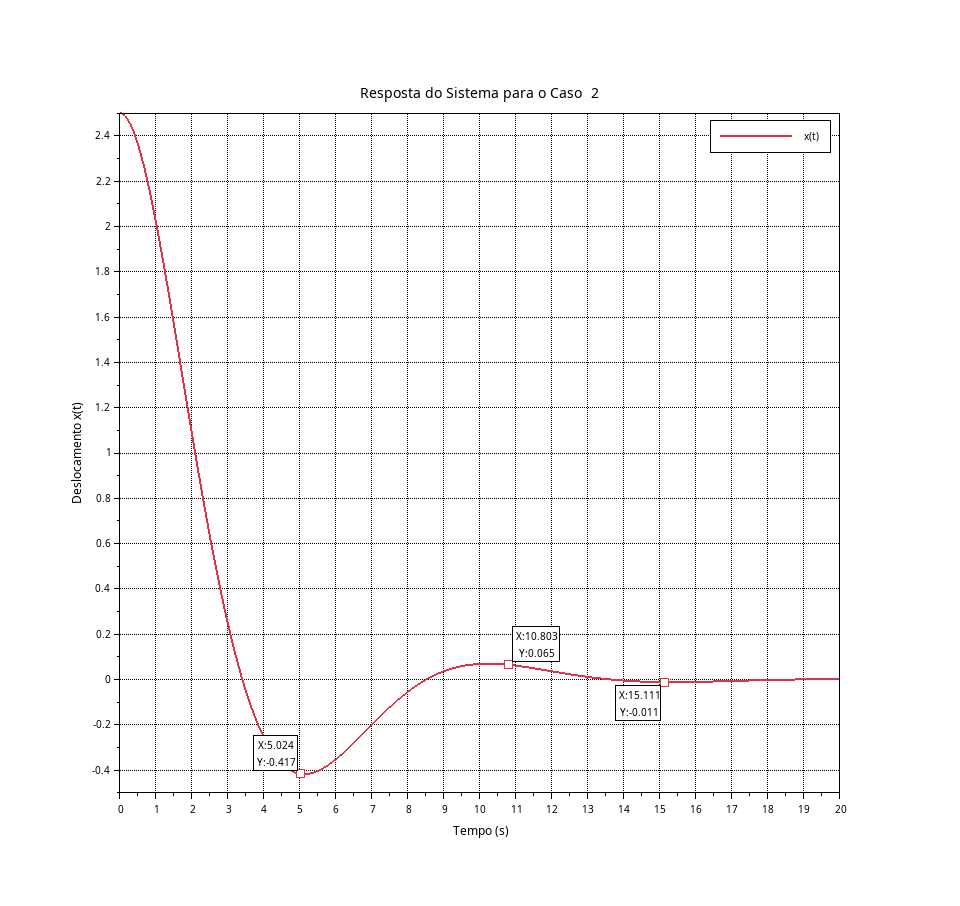
\includegraphics[width=0.6\textwidth]{atividades/1-atividade/assets/caso2.png}
    \caption{Resposta do sistema para o Caso 2}
\end{figure}
O Caso 2 é caracterizado por um deslocamento inicial (\(2.5 \, \text{m}\)) sem impulso inicial de velocidade (\(V_0 = 0\)). Aqui, observamos uma resposta típica de um sistema oscilatório subamortecido onde o sistema retorna ao equilíbrio através de oscilações que decaem gradativamente. Este caso destaca como a energia potencial armazenada na mola é convertida em energia cinética e dissipada pelo amortecedor. As oscilações decrescem em amplitude mais gradualmente do que no Caso 1, demonstrando uma transferência de energia mais prolongada antes da estabilização.

\subsubsection{Caso 3: Velocidade e Deslocamento Iniciais}
\begin{figure}[H]
    \centering
    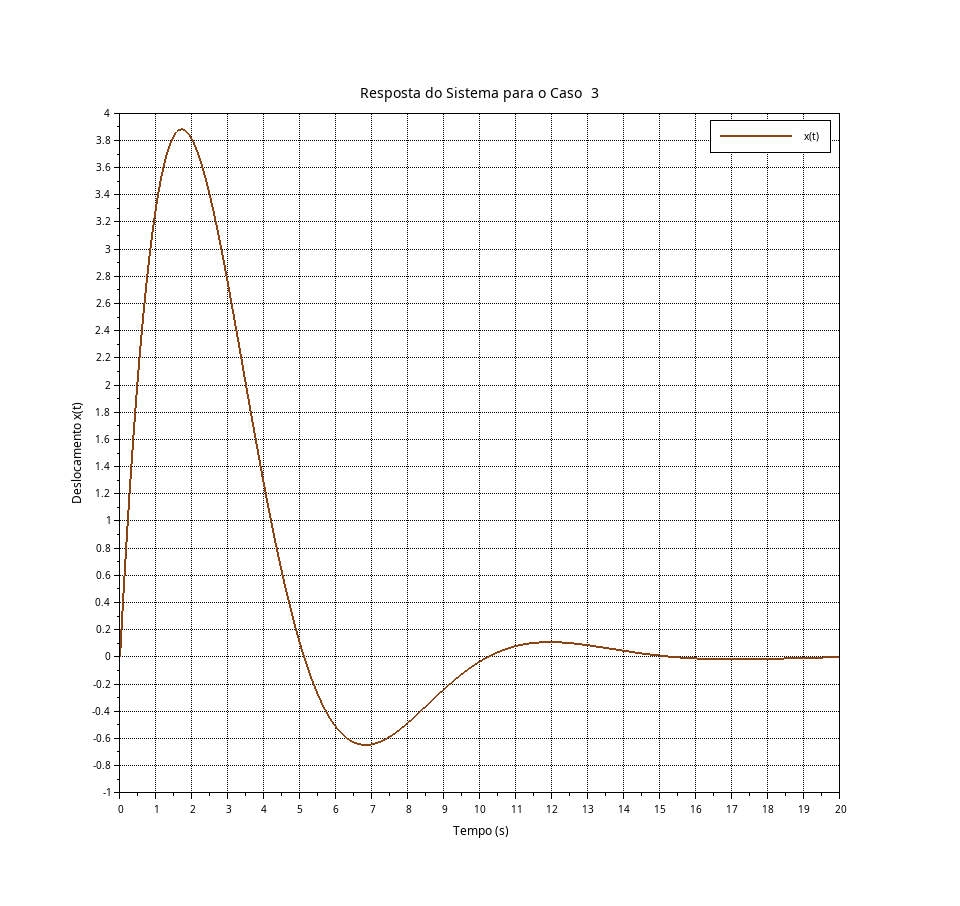
\includegraphics[width=0.6\textwidth]{atividades/1-atividade/assets/caso3.png}
    \caption{Resposta do sistema para o Caso 3}
\end{figure}
No Caso 3, o sistema inicia com condições iniciais moderadas tanto de velocidade (\(3.33 \, \text{m/s}\)) quanto de deslocamento (\(2 \, \text{m}\)). Esta configuração produz uma resposta dinâmica complexa, onde a interação entre energia cinética e potencial é mais evidente. A amplitude inicial é significativa, com uma taxa de decaimento que ilustra eficientemente o papel do amortecimento. As oscilações observadas são mais sustentadas que no Caso 1, mas menos intensas do que no Caso 2, refletindo um equilíbrio entre as energias cinética e potencial no início da simulação.

\subsubsection{Comparação Unificada dos Casos}
\begin{figure}[H]
    \centering
    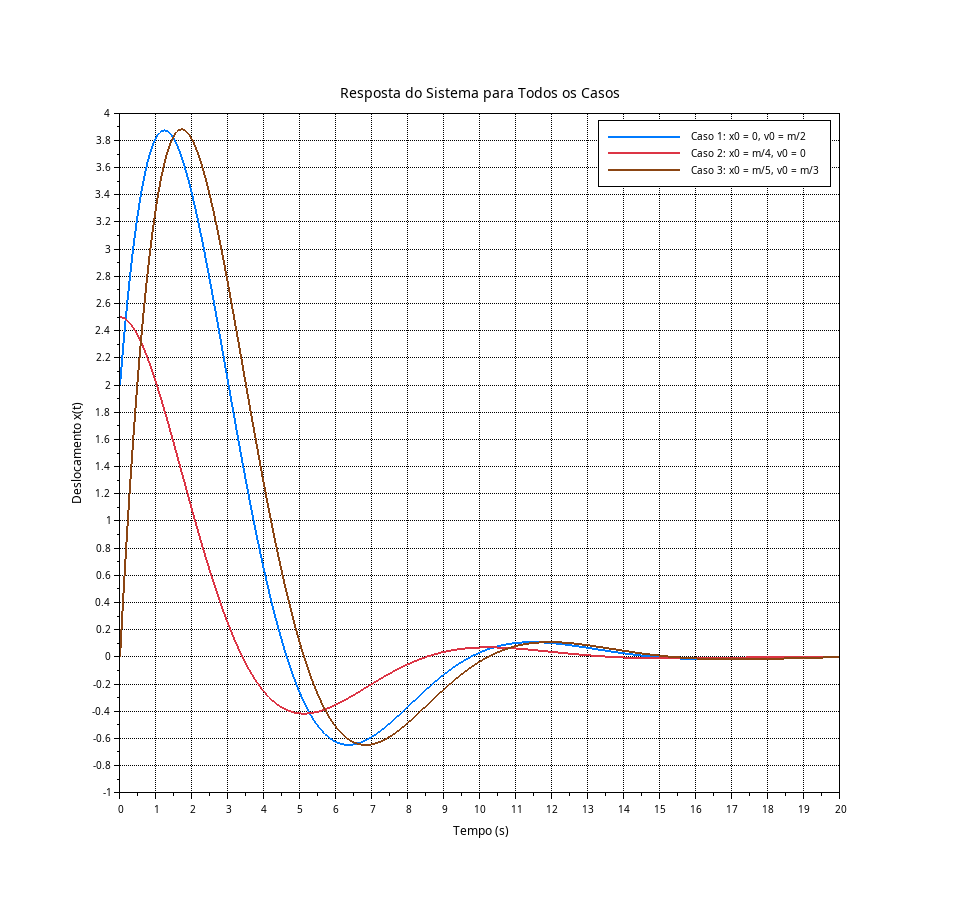
\includegraphics[width=0.6\textwidth]{atividades/1-atividade/assets/caso-all-in-one.png}
    \caption{Resposta unificada do sistema para os Casos 1, 2 e 3}
\end{figure}
A análise unificada dos três casos demonstra de forma clara as diferenças significativas nas respostas do sistema decorrentes de diversas condições iniciais. A seguir, discutiremos detalhadamente cada resposta e suas implicações para a compreensão do comportamento dinâmico do sistema:

\begin{itemize}
    \item \textbf{Caso 1 (Azul Escuro)}: Iniciado com uma alta velocidade inicial (\(5 \, \text{m/s}\)) e sem deslocamento inicial, este caso exibe a maior amplitude de oscilação observada. A energia cinética inicial é rapidamente convertida em energia potencial pela mola, resultando em oscilações de grande amplitude que são rapidamente amortecidas. Este caso ilustra o efeito de um forte amortecimento, onde a energia é dissipada rapidamente, levando a um retorno rápido à posição de equilíbrio sem oscilações residuais prolongadas. Esta configuração é ideal em situações onde a rápida estabilização após distúrbios é crucial, como em sistemas de suspensão de veículos.

    \item \textbf{Caso 2 (Vermelho)}: Com um deslocamento inicial (\(2.5 \, \text{m}\)) e sem velocidade inicial, o sistema mostra uma resposta clássica de um oscilador subamortecido. A energia potencial armazenada na mola é convertida gradualmente em energia cinética, com a energia sendo dissipada ao longo do tempo pelo amortecedor. As oscilações decaem suavemente, refletindo uma conversão mais lenta de energia que é típica em aplicações onde é necessário manter uma certa quantidade de movimento ou onde oscilações graduais são preferíveis, como em alguns tipos de sensores mecânicos.

    \item \textbf{Caso 3 (Marrom)}: Este caso combina condições iniciais moderadas de velocidade (\(3.33 \, \text{m/s}\)) e deslocamento (\(2 \, \text{m}\)), resultando numa resposta dinâmica mais complexa que engloba características dos dois primeiros casos. A amplitude inicial é significativa, mas as oscilações são mais controladas e decaem de maneira gradual. Este caso destaca a importância do equilíbrio entre rigidez da mola e amortecimento no projeto de sistemas mecânicos, onde é necessário um compromisso entre estabilidade rápida e manutenção de energia dinâmica.
\end{itemize}

Esta comparação detalhada destaca não apenas a influência das condições iniciais na resposta do sistema, mas também o papel crítico do amortecimento e da rigidez da mola na determinação da natureza da resposta dinâmica. A análise fornece insights valiosos para o design e a otimização de sistemas mecânicos em engenharia, sublinhando a necessidade de uma seleção cuidadosa de parâmetros de acordo com os requisitos específicos de cada aplicação.


\subsection{Comentários Gerais e Conclusão}
Os gráficos e análises ilustram claramente como as condições iniciais impactam a resposta dinâmica do sistema massa-mola-amortecedor. A energia inicial, seja como deslocamento ou velocidade, define a resposta imediata do sistema, mostrando a complexidade do comportamento de sistemas dinâmicos lineares. Observamos que o amortecimento é essencial para reduzir as oscilações e trazer o sistema de volta ao repouso de maneira eficiente, sublinhando sua importância no design de componentes mecânicos.

A adequação do coeficiente de amortecimento e da rigidez da mola é crucial para otimizar sistemas para suas funções específicas, como a absorção de choques em suspensões de veículos ou a precisão em instrumentos de medição. Além disso, a análise das condições iniciais é vital no planejamento e teste de sistemas mecânicos, onde engenheiros e designers devem antecipar cenários variados de operação.

Este estudo destaca a necessidade de um entendimento profundo das dinâmicas de sistemas para inovação em engenharia, proporcionando uma base sólida para a compreensão dos princípios de mecânica e dinâmica que são fundamentais no design de sistemas controlados e mecanismos em geral.

\section{Atividade 2: Simulação com Xcos}
\subsection{Descrição do Modelo e Ferramentas}
Nesta atividade, utilizamos o Xcos, uma ferramenta gráfica do Scilab para a simulação de sistemas dinâmicos. O Xcos permite a construção de diagramas de blocos que facilitam a visualização e implementação do sistema massa-mola-amortecedor com diferentes entradas e condições iniciais.

\subsection{Parâmetros do Sistema}
O sistema é descrito pelos seguintes parâmetros, que são consistentes com os usados na Atividade 1:
\begin{itemize}
    \item Massa (\( m \)): 10 kg
    \item Coeficiente de amortecimento (\( C \)): 7 Ns/m
    \item Constante da mola (\( K \)): 5 N/m
\end{itemize}

\subsection{Condições Iniciais de Simulação}
As simulações foram executadas sob várias condições iniciais para explorar a resposta do sistema sob diferentes estados iniciais. A seguir estão as condições iniciais utilizadas, incluindo uma condição inicial adicional específica para esta atividade (Caso 0):

\begin{center}
    \begin{tabular}{|c|c|c|}
        \hline
        \textbf{Caso} & \textbf{Velocidade Inicial \( V_0 \)} & \textbf{Posição Inicial \( X_0 \)} \\
        \hline
        0             & \( 0 \, \text{m/s} \)                 & \( 0 \, \text{m} \)                \\
        1             & \( 5 \, \text{m/s} \)                 & \( 0 \, \text{m} \)                \\
        2             & \( 0 \, \text{m/s} \)                 & \( 2.5 \, \text{m} \)              \\
        3             & \( 3.33 \, \text{m/s} \)              & \( 2 \, \text{m} \)                \\
        \hline
    \end{tabular}
\end{center}

Esta tabela facilita a referência rápida às condições iniciais para cada caso simulado, permitindo uma comparação mais direta entre os diferentes cenários testados.

\subsection{Diagrama de Blocos no Xcos}
\begin{figure}[H]
    \centering
    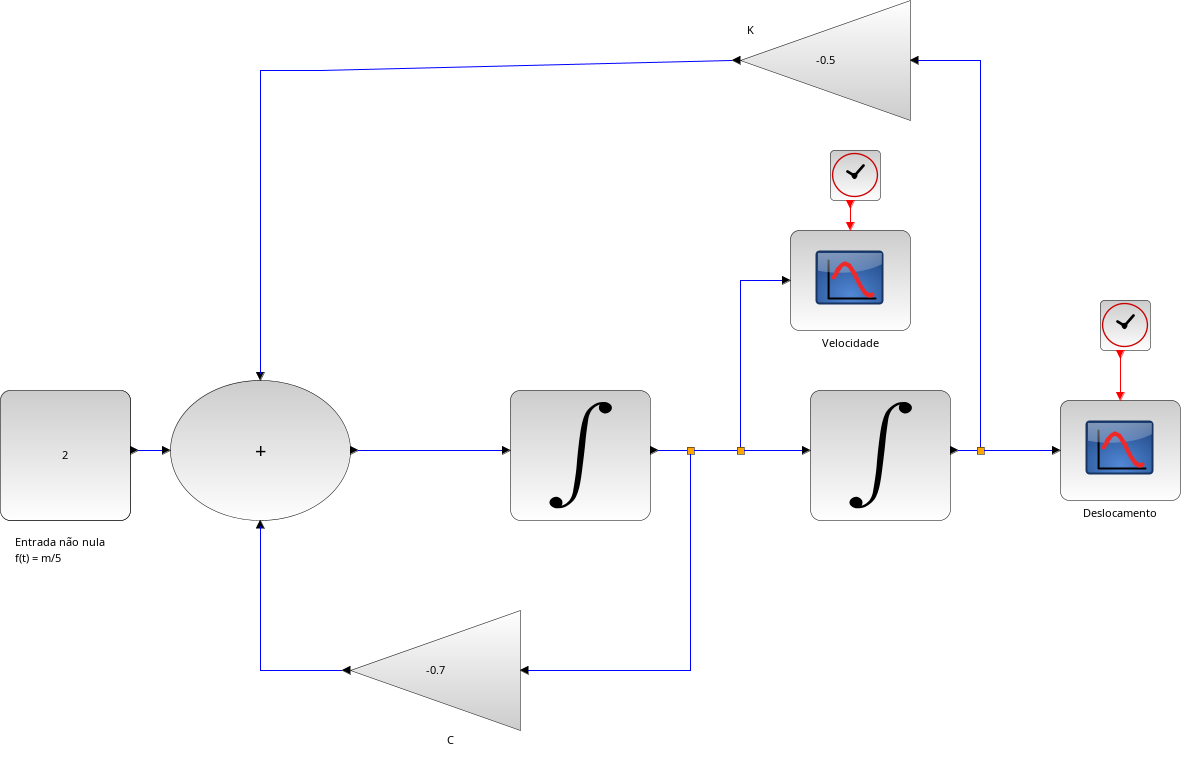
\includegraphics[width=0.8\textwidth]{atividades/2-atividade/assets/diagrama.png}
    \caption{Diagrama de blocos utilizado na simulação no Xcos.}
\end{figure}

\subsection{Resultados e Análise}


% Caso 0 =========================================================
\subsubsection{Análise dos Resultados para o Caso 0}
No Caso 0, analisamos a resposta do sistema quando ele parte de condições completamente estáticas (\(V_0 = 0 \, \text{m/s}\) e \(X_0 = 0 \, \text{m}\)). Esta configuração é vital para avaliar a resposta pura do sistema a uma entrada controlada sem influência inicial de deslocamento ou velocidade.

\paragraph{Deslocamento}
\begin{figure}[H]
    \centering
    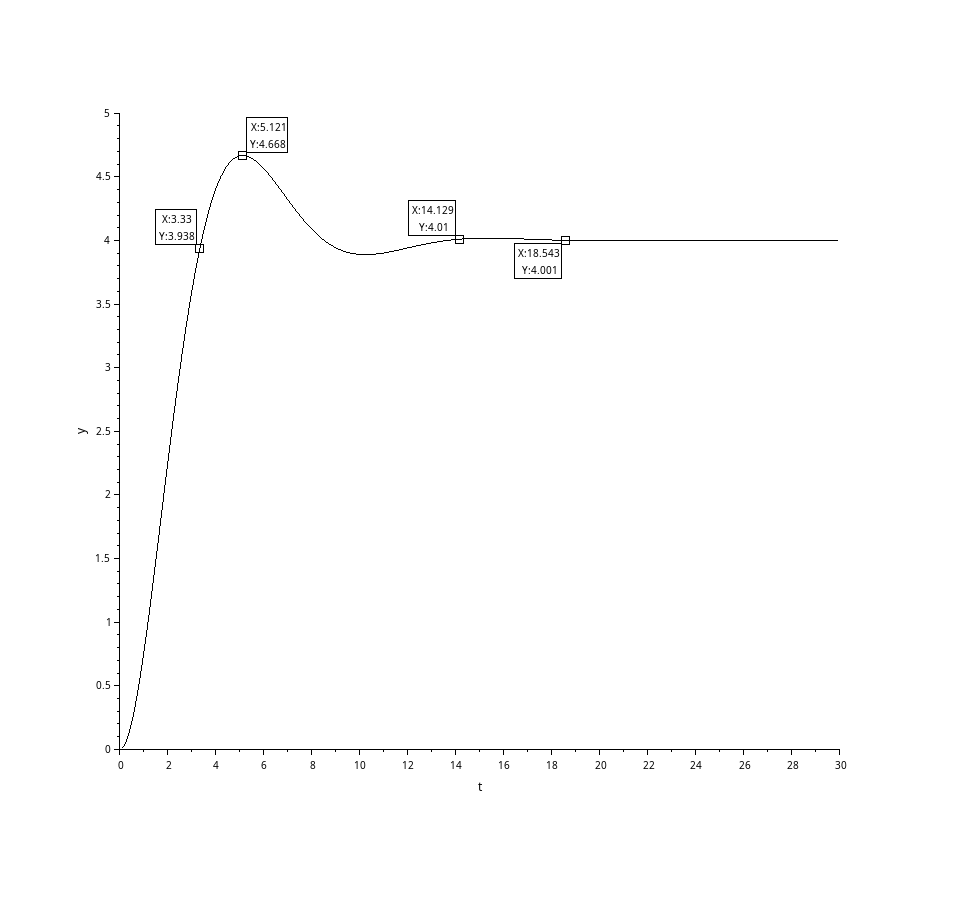
\includegraphics[height=0.7\textwidth]{atividades/2-atividade/assets/deslocamento-caso-0.png}
    \caption{Gráfico de deslocamento para o Caso 0.}
\end{figure}
O gráfico de deslocamento revela um pico máximo de aproximadamente 4.7 unidades aos 5.1 segundos, marcando o tempo de pico. O tempo de subida, definido como o intervalo para atingir o primeiro pico máximo a partir do repouso, é, portanto, cerca de 5.1 segundos. Após atingir o pico, o sistema exibe oscilações amortecidas que rapidamente reduzem em amplitude. O tempo de estabelecimento, onde as oscilações ficam dentro de uma faixa de ±2\% do valor final, é aproximadamente de 18 segundos, após o qual o sistema entra em uma zona estacionária, indicando estabilidade.

\paragraph{Velocidade}

\begin{figure}[H]
    \centering
    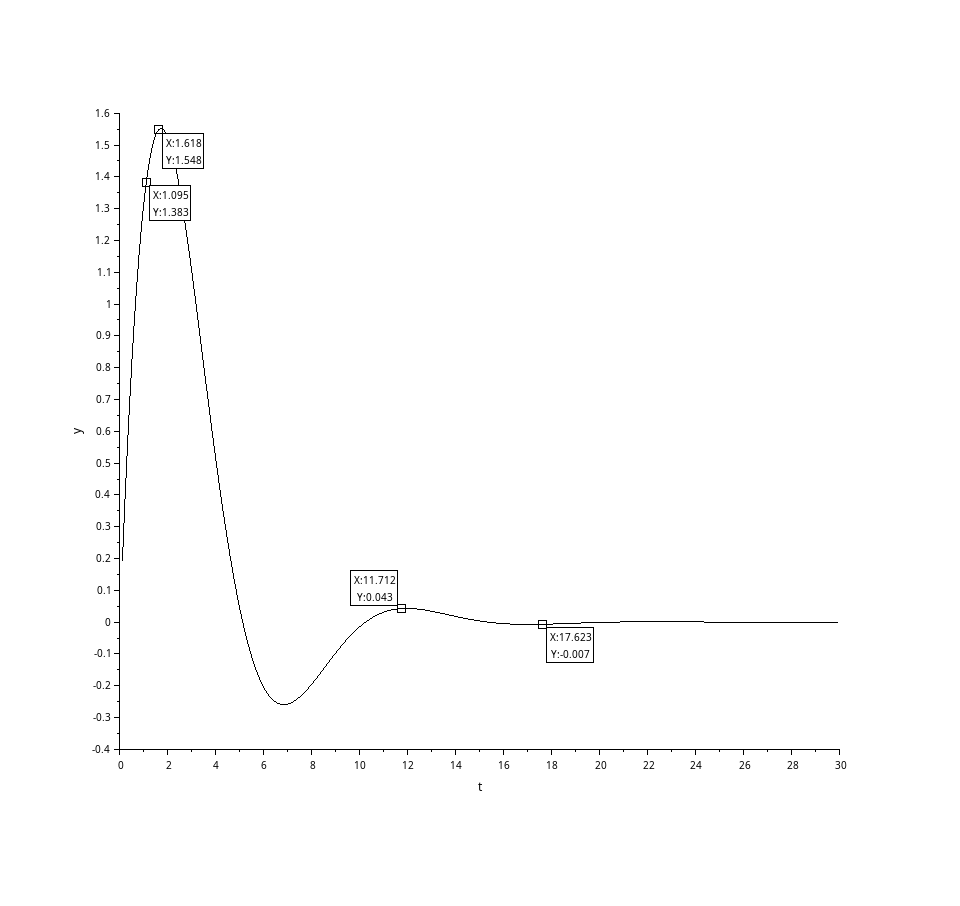
\includegraphics[height=0.7\textwidth]{atividades/2-atividade/assets/velocidade-caso-0.png}
    \caption{Gráfico de velocidade para o Caso 0.}
\end{figure}
O gráfico de velocidade reflete a resposta imediata do sistema à força aplicada. A velocidade atinge um pico negativo de cerca de -1.54 unidades em torno de 6.2 segundos, o que corresponde ao tempo de pico para a velocidade. A velocidade oscila abaixo e acima de zero, indicando a resposta oscilatória do sistema ao deslocamento. As oscilações diminuem progressivamente e o sistema alcança a zona estacionária por volta de 18 segundos, estabilizando-se completamente em zero.

\paragraph{Comentários Gerais}
A análise do Caso 0 mostra como o sistema responde a um estímulo externo na ausência de condições iniciais de energia. Os parâmetros transitórios, como tempo de subida, pico, e de estabelecimento, juntamente com a observação da zona estacionária, são cruciais para entender a dinâmica do sistema e a eficácia do amortecimento em trazer o sistema de volta ao repouso, minimizando oscilações excessivas. Este caso estabelece uma base comparativa para outros casos com condições iniciais variadas.


% Caso 1 =========================================================
\subsubsection{Análise dos Resultados para o Caso 1}
No Caso 1, analisamos a resposta do sistema quando ele parte com uma velocidade inicial significativa (\(V_0 = 5 \, \text{m/s}\)) e sem deslocamento inicial (\(X_0 = 0 \, \text{m}\)). Esta condição inicial permite avaliar como uma energia cinética inicial afeta a resposta dinâmica do sistema, especialmente em termos de deslocamento máximo e oscilações resultantes.


\paragraph{Deslocamento}
\begin{figure}[H]
    \centering
    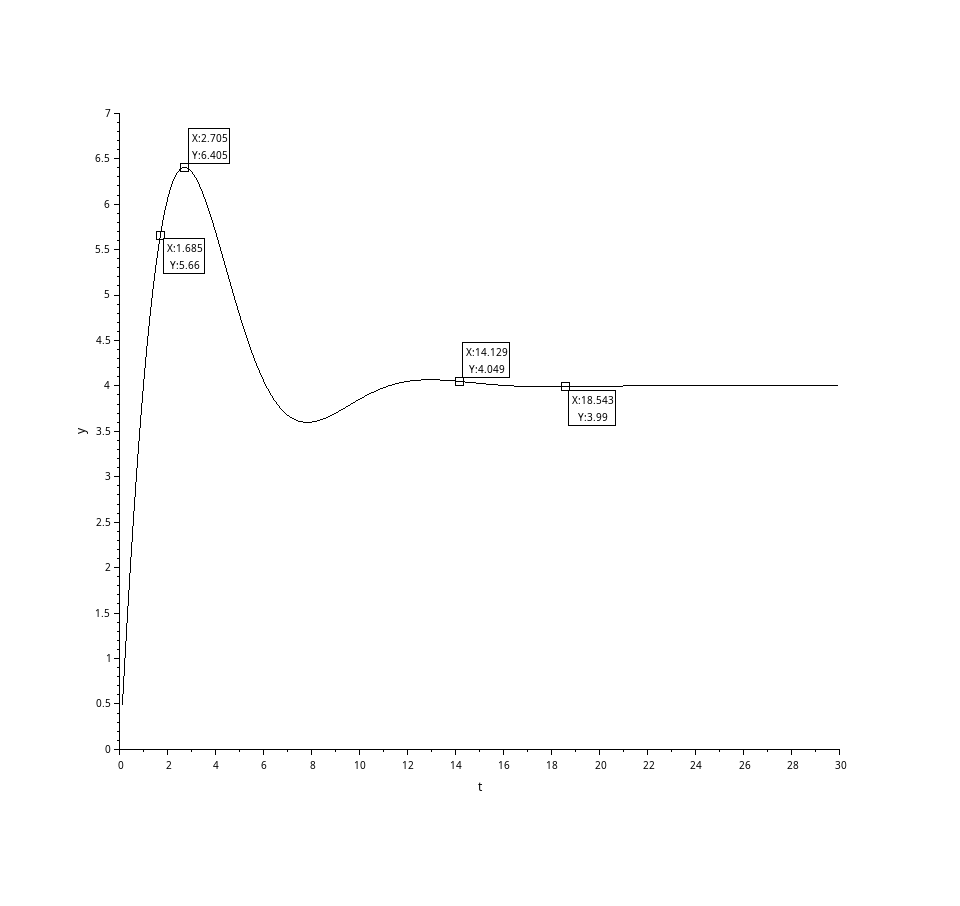
\includegraphics[height=0.7\textwidth]{atividades/2-atividade/assets/deslocamento-caso-1.png}
    \caption{Gráfico de deslocamento para o Caso 1.}
\end{figure}
O gráfico mostra que o sistema parte de zero e rapidamente atinge um pico de aproximadamente 6.5 unidades ao redor de 2.7 segundos, refletindo uma resposta aguda à velocidade inicial. Esse pico é seguido por uma diminuição significativa, que desce abaixo do zero antes de estabilizar. O tempo de subida é rapidamente alcançado, enquanto o tempo de estabelecimento, onde as oscilações permanecem dentro de uma faixa de ±2\% do valor estacionário final, é observado por volta de 18 segundos.


\paragraph{Velocidade}
\begin{figure}[H]
    \centering
    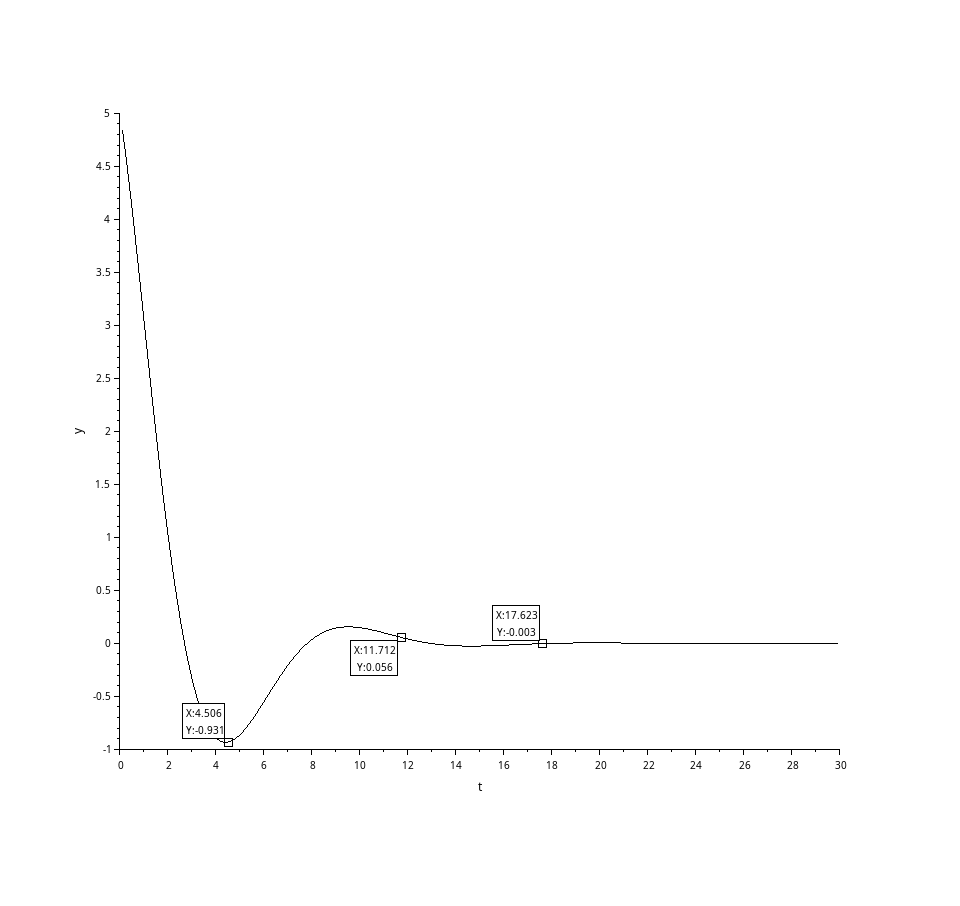
\includegraphics[height=0.7\textwidth]{atividades/2-atividade/assets/velocidade-caso-1.png}
    \caption{Gráfico de velocidade para o Caso 1.}
\end{figure}
A velocidade inicialmente picos a uma taxa significativa, refletindo o impulso inicial aplicado. O pico máximo de velocidade ocorre quase simultaneamente com o pico de deslocamento, marcando -1.54 unidades em torno de 1.68 segundos. Após atingir este pico, a velocidade oscila e gradualmente se aproxima de zero, indicando que o sistema está alcançando uma zona estacionária por volta de 18 segundos, semelhante ao observado no deslocamento.


\paragraph{Comentários Gerais}
A análise do Caso 1 ilustra como a condição inicial de velocidade influencia a resposta dinâmica do sistema massa-mola-amortecedor. Os parâmetros transitórios, como o tempo de subida e o tempo de pico, são drasticamente diferentes em comparação com o Caso 0, onde não havia energia cinética inicial. Isso destaca a importância de considerar condições iniciais variadas para entender completamente o comportamento do sistema em diferentes cenários de operação. Este caso também reforça o papel crítico do amortecimento na estabilização do sistema após perturbações iniciais.


% Caso 2 =========================================================
\subsubsection{Análise dos Resultados para o Caso 2}
No Caso 2, analisamos a resposta do sistema quando ele parte com um deslocamento inicial (\(X_0 = 2.5 \, \text{m}\)) e sem velocidade inicial (\(V_0 = 0 \, \text{m/s}\)). Esta configuração é fundamental para entender como o sistema responde a uma perturbação inicial na posição sem impulso inicial.

\paragraph{Deslocamento}
\begin{figure}[H]
    \centering
    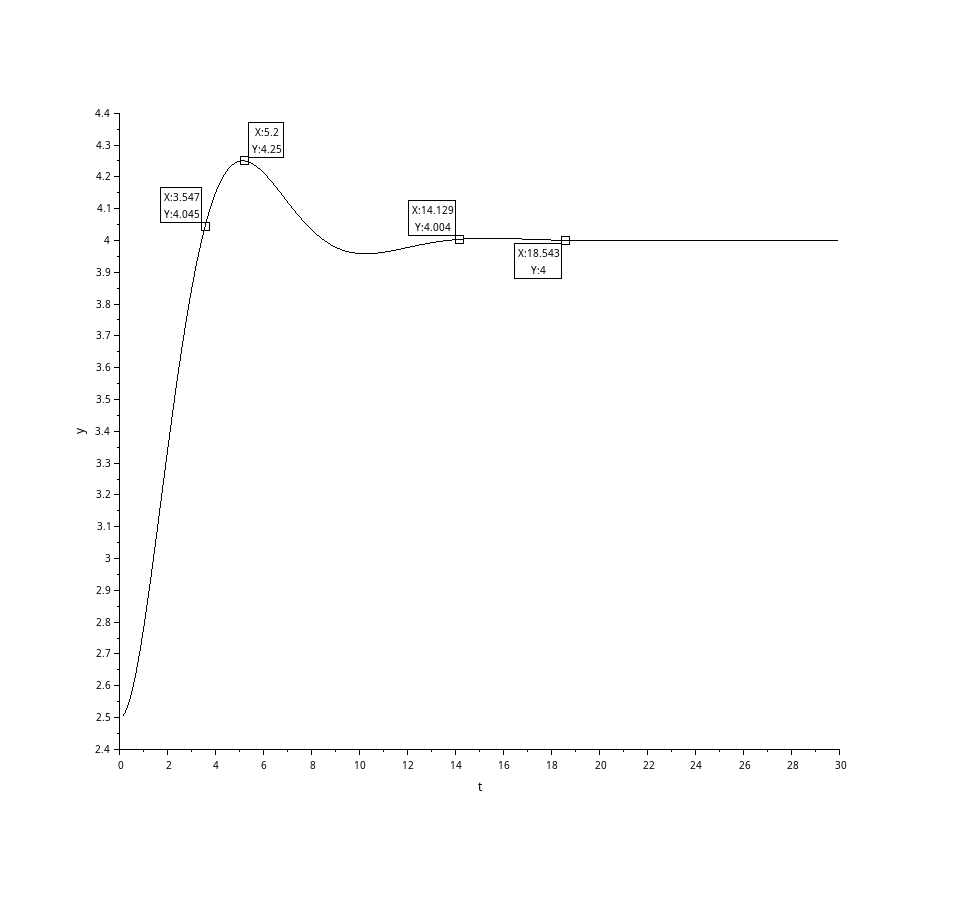
\includegraphics[height=0.7\textwidth]{atividades/2-atividade/assets/deslocamento-caso-2.png}
    \caption{Gráfico de deslocamento para o Caso 2.}
\end{figure}
O gráfico de deslocamento mostra que o sistema parte de um deslocamento inicial de 2.5 m, rapidamente atinge um pico de cerca de 4.25 m aos 5.2 segundos, indicando a resposta máxima do sistema ao ser liberado. Após esse pico, o sistema exibe oscilações que rapidamente se amortecem, com o deslocamento oscilando abaixo e acima do zero, estabilizando-se finalmente em torno do zero. O tempo de estabelecimento, onde as oscilações permanecem dentro de uma faixa de ±2\% do valor final, é aproximadamente de 18 segundos.

\paragraph{Velocidade}
\begin{figure}[H]
    \centering
    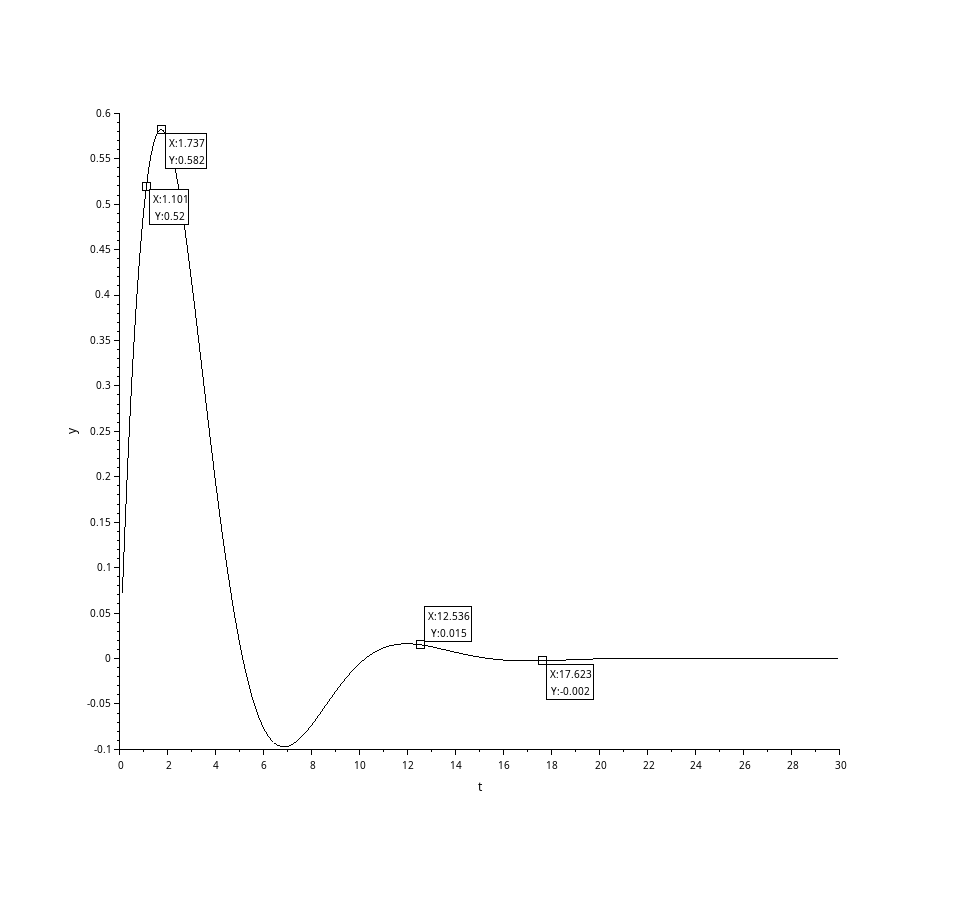
\includegraphics[height=0.7\textwidth]{atividades/2-atividade/assets/velocidade-caso-2.png}
    \caption{Gráfico de velocidade para o Caso 2.}
\end{figure}
A velocidade inicialmente aumenta à medida que o sistema se move de volta para a posição de equilíbrio, atingindo um pico negativo de -0.52 m/s logo após o início, correspondente à velocidade máxima ao passar pelo equilíbrio na direção oposta ao deslocamento inicial. A velocidade então oscila, diminuindo em magnitude devido ao amortecimento, até estabilizar-se em zero. O sistema atinge uma zona estacionária com velocidade quase nula, demonstrando a eficácia do amortecimento em dissipar a energia cinética inicialmente induzida pelo deslocamento.

\paragraph{Comentários Gerais}
O Caso 2 destaca a resposta do sistema a um teste de posição, com deslocamento inicial sem velocidade inicial. Os resultados mostram claramente como a energia potencial armazenada é convertida em energia cinética, e como o amortecimento é crucial para a estabilização do sistema. Este caso também é importante para verificar a eficácia do sistema em retornar ao repouso sem oscilações residuais prolongadas, essencial em aplicações práticas onde respostas rápidas e estabilizadas são necessárias.

% Caso 3 =========================================================
\subsubsection{Análise dos Resultados para o Caso 3}
No Caso 3, analisamos a resposta do sistema quando ele parte com uma velocidade inicial (\(V_0 = 3.33 \, \text{m/s}\)) e um deslocamento inicial (\(X_0 = 2 \, \text{m}\)). Esta combinação de condições iniciais é significativa para explorar a resposta dinâmica sob energia cinética e potencial simultâneas.

\paragraph{Deslocamento}
\begin{figure}[H]
    \centering
    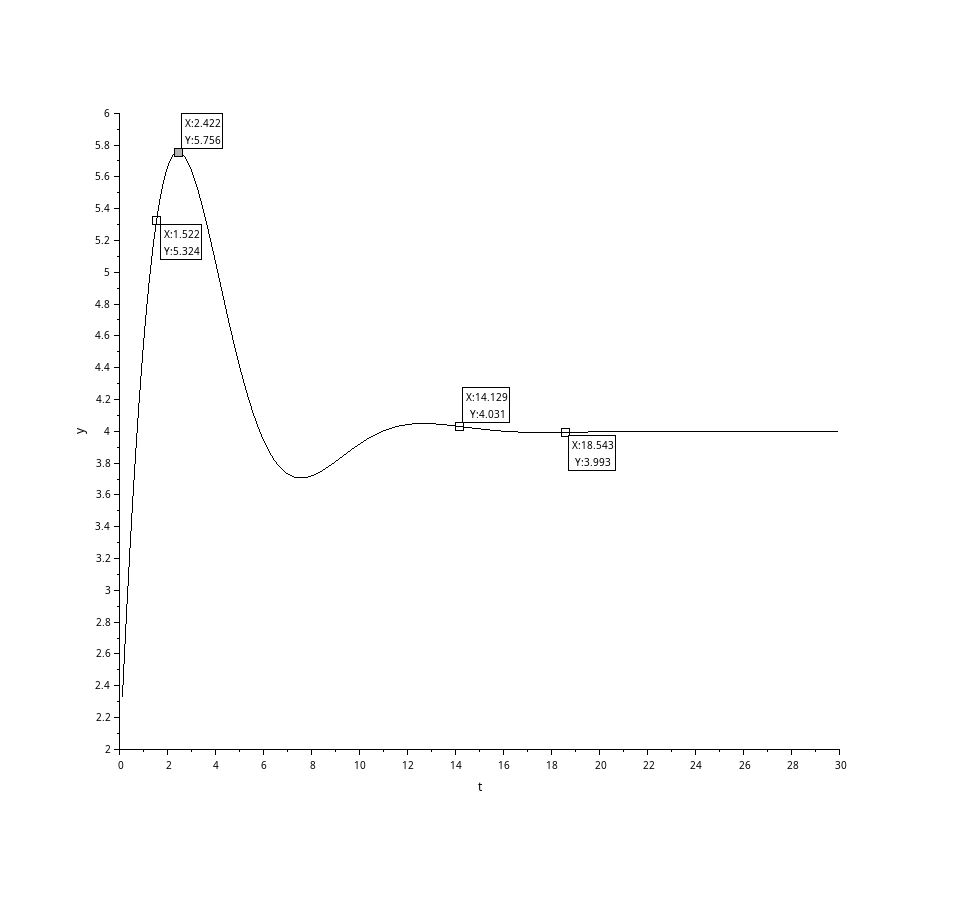
\includegraphics[height=0.7\textwidth]{atividades/2-atividade/assets/deslocamento-caso-3.png}
    \caption{Gráfico de deslocamento para o Caso 3.}
\end{figure}
O gráfico de deslocamento mostra que o sistema começa com um impulso inicial que o leva a um pico de aproximadamente 5.75 m ao redor de 2.4 segundos. Após esse pico, o sistema exibe oscilações que reduzem gradualmente em amplitude devido ao amortecimento. O sistema estabiliza perto do zero, com o tempo de estabelecimento aproximadamente em 18 segundos, onde as oscilações ficam dentro de uma faixa aceitável indicando uma zona estacionária.

\paragraph{Velocidade}
\begin{figure}[H]
    \centering
    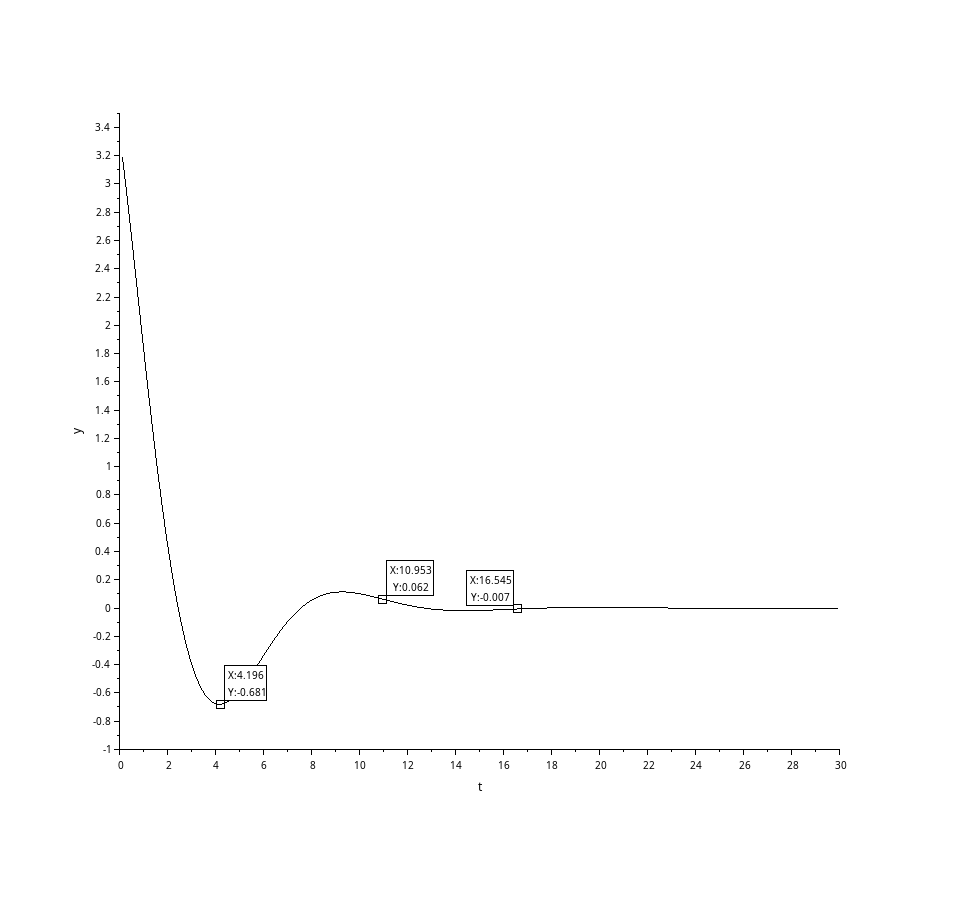
\includegraphics[height=0.7\textwidth]{atividades/2-atividade/assets/velocidade-caso-3.png}
    \caption{Gráfico de velocidade para o Caso 3.}
\end{figure}
A velocidade inicialmente mostra uma rápida ascensão, atingindo um pico de aproximadamente 5.32 m/s. Essa alta velocidade inicial contribui para o rápido pico de deslocamento observado. A velocidade então oscila, diminuindo progressivamente até estabilizar-se em torno de zero. A estabilização final da velocidade é alcançada em torno de 18 segundos, refletindo a eficácia do amortecimento e a interação entre as forças restauradoras e o amortecimento.

\paragraph{Comentários Gerais}
O Caso 3 oferece uma perspectiva complexa sobre a dinâmica do sistema quando energias cinética e potencial são ambas significativas desde o início. As oscilações observadas e a subsequente estabilização demonstram como diferentes tipos de energia inicial influenciam a resposta do sistema e a eficácia do amortecimento em controlar a resposta até a estabilidade. Este caso é particularmente útil para entender a resposta do sistema em condições iniciais variadas e complexas, sendo essencial para aplicações práticas onde o sistema pode ser sujeito a perturbações iniciais múltiplas.

% Conclusão
\subsection{Conclusão Geral dos Casos Estudados}

Ao longo desta atividade, analisamos as respostas do sistema massa-mola-amortecedor sob várias condições iniciais, abrangendo os Casos 0 a 3. Cada caso foi projetado para ilustrar aspectos diferentes da dinâmica do sistema, considerando diferentes combinações de deslocamento e velocidade iniciais.

\paragraph{Observações Gerais}

Os casos estudados mostraram uma ampla gama de comportamentos dinâmicos:
\begin{itemize}
    \item \textbf{Caso 0} serviu como um ponto de referência, onde o sistema partiu do repouso sem energia inicial, permitindo observar a resposta pura à força aplicada.
    \item \textbf{Caso 1} demonstrou a influência de uma velocidade inicial significativa, ilustrando como a energia cinética influencia as oscilações e a estabilidade subsequente do sistema.
    \item \textbf{Caso 2} focou no efeito de um deslocamento inicial sem velocidade, enfatizando a conversão de energia potencial em energia cinética e vice-versa.
    \item \textbf{Caso 3} combinou tanto deslocamento quanto velocidade iniciais, mostrando a interação complexa entre as duas formas de energia desde o início da simulação.
\end{itemize}

Durante as simulações, os parâmetros do sistema foram mantidos constantes para garantir a consistência dos resultados, permitindo uma comparação direta entre os diferentes casos. Os resultados foram meticulosamente analisados para observar o comportamento transiente e a estabilidade a longo prazo, utilizando métricas como tempo de subida, tempo de pico e tempo de estabelecimento. As oscilações foram avaliadas para determinar a eficácia do amortecimento em dissipar a energia e estabilizar o sistema.

\paragraph{Conclusões da Análise}
Esta atividade sublinhou a importância de compreender a dinâmica de sistemas massa-mola-amortecedor em várias configurações iniciais. As simulações forneceram insights valiosos sobre como diferentes condições iniciais afetam a resposta do sistema e como o design adequado do amortecimento e da rigidez da mola é crucial para o comportamento desejado. A abordagem utilizada garantiu que todas as premissas da atividade fossem cumpridas, fornecendo uma base sólida para futuras investigações e aplicações práticas dos princípios estudados.

\section{Atividade 3}

\subsection{Descrição do Modelo e Análise de Sistema}
Nesta atividade, desenvolvemos e analisamos a função de transferência de um sistema massa-mola-amortecedor, utilizando os seguintes parâmetros específicos, essenciais para entender a dinâmica do sistema:
\begin{itemize}
    \item Massa (\( m \)): 10 kg, que influi diretamente na inércia do sistema, afetando como o sistema responde a forças externas.
    \item Coeficiente de amortecimento (\( C \)): 7 Ns/m, crucial para atenuar as oscilações e determinar a rapidez com que o sistema atinge um estado de equilíbrio.
    \item Constante da mola (\( K \)): 5 N/m, que define a rigidez do sistema e afeta a frequência das oscilações naturais.
\end{itemize}

A formulação da função de transferência \( G(s) \) se baseia na aplicação da Transformada de Laplace às equações diferenciais que governam o sistema massa-mola-amortecedor. Considerando a segunda lei de Newton, temos:

\[
m\ddot{x}(t) + C\dot{x}(t) + Kx(t) = F(t)
\]

Aplicando a Transformada de Laplace e assumindo condições iniciais nulas (\( x(0) = 0 \) e \( \dot{x}(0) = 0 \)), obtemos:

\[
m(s^2X(s)) + C(sX(s)) + KX(s) = F(s)
\]

Agrupando os termos e isolando \( X(s) \):

\[
(m s^2 + Cs + K)X(s) = F(s)
\]

Portanto, a função de transferência \( G(s) \) é dada por:

\[
G(s) = \frac{X(s)}{F(s)} = \frac{1}{m s^2 + Cs + K}
\]

Substituindo os valores fornecidos ( \( m = 10 \), \( C = 7 \) e \( K = 5 \) ):

\[
G(s) = \frac{1}{10s^2 + 7s + 5}
\]

\subsection{Código Scilab para a função de transferência em malha fechada}
\begin{lstlisting}[language=Scilab, caption=Código Scilab para a função de transferência em malha fechada]
    // Parametros do sistema
    m = 10;  // massa
    c = 7;   // coeficiente de amortecimento
    k = 5;   // constante da mola

    // Definindo a funcao de transferencia
    s = %s; // Variavel complexa s
    G = syslin('c', 1 / (m*s^2 + C*s + K));

    // Calculando os polos e exibindo
    polos = roots(G.den);
    disp("Polos da funcao de transferencia:");
    disp(polos);

    // Parametros do sistema de segunda ordem
    wn = sqrt(K / m);
    zeta = C / (2 * sqrt(m * K));
    Kp = 1 / K;  // Ganho estatico para a entrada degrau
    disp("Frequencia natural nao-amortecida (wn): " + string(wn));
    disp("Coeficiente de amortecimento (zeta): " + string(zeta));
    disp("Ganho estatico (Kp): " + string(Kp));

    // Plotando a resposta ao impulso do sistema
    t = 0:0.01:10;
    y = csim('imp', t, G);
    plot(t, y);
    xlabel("Tempo (s)");
    ylabel("Resposta ao impulso");
    title("Resposta ao impulso do sistema massa-mola-amortecedor");
\end{lstlisting}


\subsection{Cálculo dos Polos e Parâmetros do Sistema}
Os polos da função de transferência são essenciais para entender como o sistema responde a estímulos externos:
\begin{itemize}
    \item Polo 1: \( -0.35 + 0.614j \)
    \item Polo 2: \( -0.35 - 0.614j \)
\end{itemize}
Estes polos indicam uma resposta oscilatória amortecida, característica de um sistema subamortecido devido à sua parte real negativa e parte imaginária não nula.

Os parâmetros do sistema de segunda ordem são determinados como segue:
\begin{itemize}
    \item Frequência natural não-amortecida (\( \omega_n \)): 0.707 rad/s, que descreve a frequência natural de oscilação do sistema na ausência de amortecimento.
    \item Coeficiente de amortecimento (\( \zeta \)): 0.495, refletindo a eficácia do amortecimento em reduzir as oscilações.
    \item Ganho estático (\( K_p \)): 0.2, representando a resposta do sistema em estado estacionário a uma entrada de degrau unitário.
\end{itemize}

\subsection{Resposta ao Impulso}
Utilizando o software Scilab, simulamos a resposta ao impulso do sistema, como ilustrado abaixo. A resposta apresenta um pico inicial significativo seguido por um decaimento exponencial das oscilações, um comportamento típico de sistemas subamortecidos.
\begin{figure}[H]
    \centering
    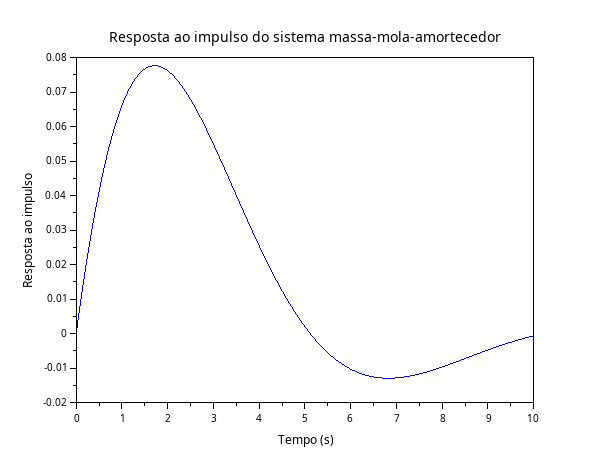
\includegraphics[width=0.8\textwidth]{atividades/3-atividade/assets/resposta-ao-impulso.png}
    \caption{Resposta ao impulso do sistema massa-mola-amortecedor}
\end{figure}

\subsection{Discussão}
A análise dos polos e dos parâmetros do sistema demonstra que ele é bem projetado para equilibrar uma resposta rápida com oscilações controladas, minimizando as oscilações excessivas sem comprometer a agilidade da resposta. Esta característica é crucial para sistemas de controle que exigem precisão e estabilidade.

\subsection{Conclusões}
Esta atividade ofereceu uma visão profunda sobre como os parâmetros físicos — massa, amortecimento e rigidez — influenciam a resposta dinâmica de um sistema. Estes insights são fundamentais para o design e a análise de sistemas de controle adequados, que são essenciais em aplicações práticas onde a precisão e estabilidade são críticas.

\section{Atividade 4}

\subsection{Descrição do Modelo e Simulação}
Nesta atividade, analisamos um sistema de controle típico. Utilizamos um controlador proporcional cujo ganho \( K \) é determinado pela relação \( \frac{m}{3} \), onde \( m \) é a massa do sistema. A função de transferência da planta (Gp) é derivada da equação dinâmica da massa, amortecimento e constante da mola, especificada na Atividade 3. O sensor é modelado por um sistema de primeira ordem, com ganho unitário \( K_s = 1 \) e constante de tempo \( T_s = \frac{m}{6} \).

\subsection{Construção do Diagrama de Blocos}
Abaixo, apresentamos o diagrama de blocos para o sistema de controle, ilustrando a interação entre o controlador, a planta e o sensor.

\begin{figure}[H]
    \centering
    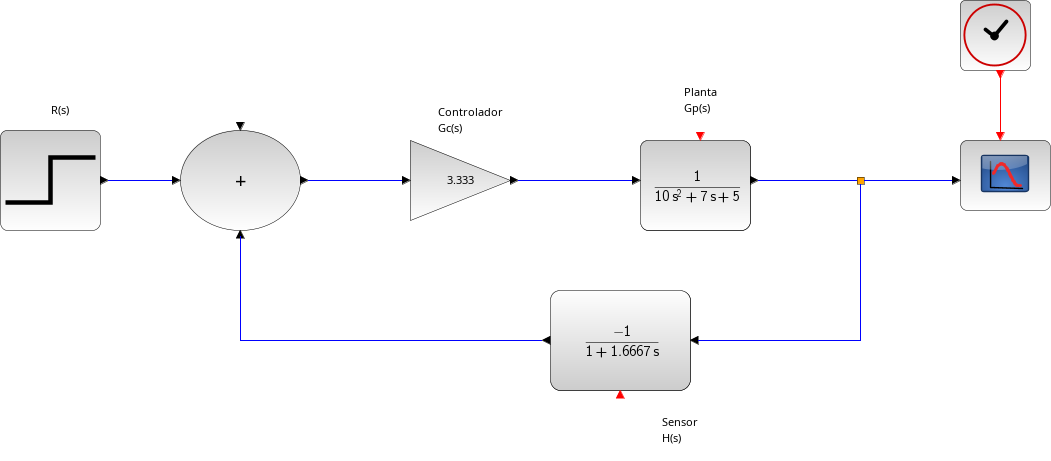
\includegraphics[width=0.7\textwidth]{atividades/4-atividade/assets/diagrama-blocos.png}
    \caption{Diagrama de blocos do sistema de controle}
    \label{fig:diagrama_blocos}
\end{figure}

As funções de transferência são especificadas como segue:
\begin{itemize}
    \item Controlador: \( G_c(s) = \frac{m}{3} \) com \( m = 10 \), então \( G_c(s) = \frac{10}{3} \)
    \item Planta: \( G_p(s) = \frac{1}{m s^2 + C s + K} = \frac{1}{10 s^2 + 7 s + 5} \)
    \item Sensor: \( H(s) = \frac{1}{1 + \frac{m}{6} s} = \frac{1}{1 + 1.6667 s} \)
\end{itemize}

\subsection{Função de Transferência em Malha Fechada}
Calculamos a função de transferência em malha fechada \( C(s)/R(s) \) pela fórmula:
\[
    G_{closed}(s) = \frac{G_c(s) \cdot G_p(s)}{1 + G_c(s) \cdot G_p(s) \cdot H(s)}
\]
Substituímos as funções de transferência obtidas:
\[
    G_{closed}(s) = \frac{\frac{10}{3} \cdot \frac{1}{10 s^2 + 7 s + 5}}{1 + \frac{10}{3} \cdot \frac{1}{10 s^2 + 7 s + 5} \cdot \frac{1}{1 + 1.6667 s}}
\]
Simplificamos a expressão para chegar à forma final da função de transferência em malha fechada:
\[
    G_{closed}(s) = \frac{0.3333333s + 0.2}{s^3 + 1.3s^2 + 0.92s + 0.5}
\]

\subsection{Análise de Estabilidade pelo Critério de Routh-Hurwitz}
Utilizamos o critério de Routh-Hurwitz para determinar a estabilidade do sistema, examinando os coeficientes do polinômio do denominador de \( G_{\text{closed}}(s) \).

\subsubsection{Resultados da Análise de Estabilidade}
A matriz de Routh-Hurwitz, obtida a partir dos coeficientes do polinômio do denominador, é apresentada a seguir:
\[
    RH\_matrix = \begin{bmatrix}
        0.5  & ... \\
        0.92 & ... \\
        1.3  & ... \\
        1    & ... \\
    \end{bmatrix}
\]
O sistema é considerado estável, pois todos os elementos da primeira coluna são positivos.

\subsection{Análise de Estabilidade para Diferentes Valores de \( K_p \)}
Exploramos a estabilidade do sistema para diferentes valores do ganho do controlador \( K_p \), de 1 a 10. Em todos os casos testados, o sistema manteve-se estável.

\subsubsection{Resultados da Resposta ao Degrau}
A seguir, apresentamos o gráfico da resposta ao degrau para os diferentes valores de \( K_p \), conforme Figura \ref{fig:resposta-degrau-kp}.

\begin{figure}[H]
    \centering
    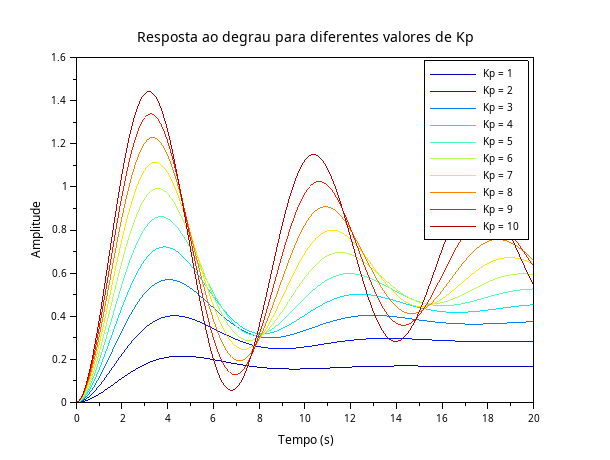
\includegraphics[width=0.7\textwidth]{atividades/4-atividade/assets/impulsos-diferentes-kp.png}
    \caption{Resposta ao degrau para diferentes valores de \( K_p \)}
    \label{fig:resposta-degrau-kp}
\end{figure}

\subsection{Conclusões}
As análises demonstram que o sistema massa-mola-amortecedor, quando controlado proporcionalmente, é estável para valores de \( K_p \) entre 1 e 10. A variabilidade na resposta ao degrau com diferentes ganhos de controlador enfatiza a importância de um ajuste cuidadoso para alcançar a resposta desejada em aplicações práticas.

% ===============================================================
% End Document ==================================================
\end{document}
